\section{模型准备}\label{sec:preparation}
本章统一后续各问的几何对象、空间变量与径向抽象。几何基础可以共用，但物性关系、环境边界及求解目标仍由各问确定；一维近似的适用程度也须结合相应时段与目标检验。
\subsection{一维近似的几何与尺度依据}
\textbf{（1）侧面交换面积占主导，为径向一维建模提供几何依据。}
令$A_{\rm e}$为两个端面的总面积、$A_{\rm s}$为侧面积、$A_{\rm tot}$为总表面积，单位均为m$^2$。由圆柱几何关系，
\[
A_{\rm e}=2\pi R^2,\qquad A_{\rm s}=2\pi RL,\qquad
\frac{A_{\rm s}}{A_{\rm tot}}=\frac{L}{L+R}=\frac{25}{27}\approx92.59\%,
\qquad \frac{A_{\rm e}}{A_{\rm s}}=\frac RL=0.08.
\]
若端面和侧面的交换系数相同，且相应的平均温差或水分驱动力处于同一数量级，而侧面积约占总面积的比重92.59\%，因此以侧面交换为主建立模型。

\textbf{（2）径向与轴向特征长度存在分离。}
取半径$R$和半长$H$作为径向、轴向特征长度，引入无量纲坐标$\xi=r/R$、$\zeta=z/H$。对温度或含水率的代表场$u$，以局部常系数扩散算子说明尺度关系：
\[
\frac1r\partial_r(r\partial_r u)+\partial_z^2u
=\frac1{R^2}\left[\frac1\xi\partial_\xi(\xi\partial_\xi u)
+\left(\frac RH\right)^2\partial_\zeta^2u\right],
\qquad \left(\frac RH\right)^2=0.0256.
\]
当两方向采用相同的有效传递系数，且无量纲场在两方向的曲率量级相近时，轴向项具有较小的几何系数，因而径向主导是合理的初始近似。


\subsection{建模对象与径向抽象}
题给药材半径$R=0.02$~m、全长$L=0.25$~m，半长$H=L/2=0.125$~m。取单位轴向长度的药材截面，径向范围为$0\le r\le R$，待求状态为温度$\theta_1(r,t)$与干基含水率$C_1(r,t)$。外界变化通过侧面对流换热和水分交换传入材料，内部状态随半径变化。根据5.1分析，仅保留径向梯度建立一维模型。

在均质圆柱、初始状态周向均匀、侧面环境与交换参数周向一致的假设下，状态不依赖周向角，空间描述可先简化为轴对称的$(r,z)$二维问题。

\begin{figure}[H]\centering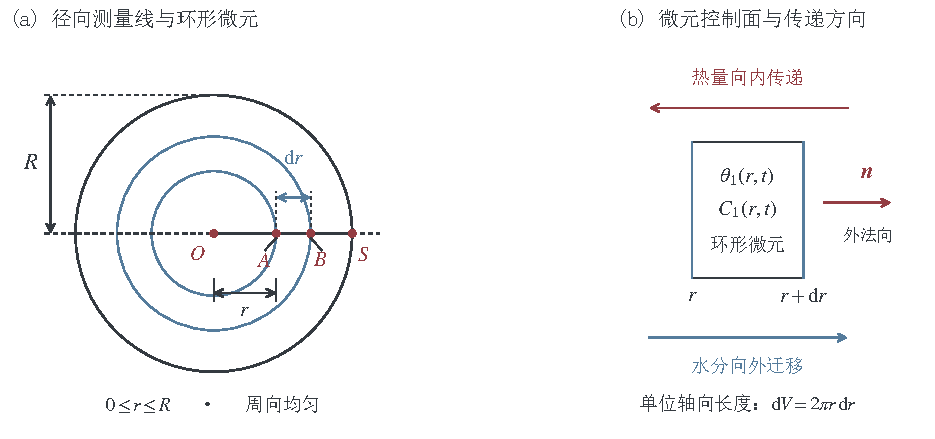
\includegraphics[width=\textwidth]{figures/q1_radial_geometry.pdf}
\caption{径向测量线与环形微元}\label{fig:radial}\end{figure}
图\ref{fig:radial}(a)以轴心$O$、侧面点$S$确定径向测量线，$A,B$标记半径$r$、$r+dr$处的微元边界，$dr$为微小径向厚度；(b)示意微元内、外控制面及典型升温脱水阶段的热量内传、水分外迁方向。图中$\boldsymbol n$为沿径向向外的单位法向量，环厚为清晰起见放大；单位轴向长度的环形微元体积在一阶微分意义下为$dV=2\pi r\,dr$，为后续守恒方程提供几何基础。



\subsection{近似的使用约定与检验边界}
上述理由共同支持先建立一维径向主模型，再用二维轴对称模型量化忽略轴向传递造成的变化。一维场$\theta_1(r,t),C_1(r,t)$是降维模型的输出，不预先定义为二维中截面真值或全长平均值。中截面远离两端，适合作为交叉比较的位置，但对称性仅保证$\partial_z u(r,0,t)=0$，并不保证$\partial_z^2u(r,0,t)=0$，所以中截面仍可能受轴向传递影响。

比较时应保持径向网格、环境输入及径向物性处理一致，同时检查中截面、端部与整体目标量。温度和水分的特征扩散率不同，二者须分别检验；某一时段中截面的差异较小，不能外推为端面、全体积或后续长时过程同样准确。本文沿用一维模型给出正式结果，二维模型用于误差说明；具体差值与适用范围见各问的模型检验。涉及终止时间等全域目标时，还须比较目标量本身，不能仅以中截面的场值差作为依据。
